\section{Usability of EvoSuite}

In this section, we briefly explore the usability of EvoSuite.
Automated test case generation is a real solution for the burden software testing can be. 
But if a tool like EvoSuite that provides such automation is difficult to use, it does not add much ease to the process of testing. 
We provide with a report on problems encountered when using the tool on Microsoft Windows 10, and on further issues concerning Maven and EvoSuite. 

\subsection{Problems Encountered}

In this part, we report the issues that we encountered during installation and working with automated test generation tool EvoSuite. 
The operating system is Microsoft Windows 10, 64bit. 
After a proper installation, according to the guidelines from the official site \verb|http://www.evosuite.org/| and choosing one of the different ways to execute a test generation tool, namely run EvoSuite from the command line. 
The tool is assembled and compiled in an independent executable jar (e.g., \verb|evosuite.jar|). 
The CUT that we have chosen is Joda-Time that provides API that replaces the standard Java date and time classes. 
However, we discovered a problem on one of the working stations after invoking the given command: 

\verb|$ java -jar evosuite.jar -generateSuite -projectCP <class_path> -class <class_name>|,

where the option \-class is used to define the CUT, and the option -projectCP is used to indicate the classpath.
The error message is shown in figure \ref{fig:error}.

Theoretically, if the correct path is provided, this approach is supposed to work fine if EvoSuite is specified in a "static" context, e.g., when the class path does not change, and a user only changes the CUT's file name.
The installed version of JDK is \verb|1.8.0_60|. 
The system and user variables of the system are defined as follows: \verb|JAVA_HOME| variable is set at \verb|jdk1.8.0_60| and \verb|PATH| at \verb|jdk1.8.0_60/bin|.
However, one of the possible reasons for triggering that error was the assumption that the User Environment variables were not properly set. 
The \verb|PATH| and \verb|JAVA_HOME| variable were excluded from the system variables list but apparently that did not lead to a positive outcome and the possibility to run the test suite to the end. 
Before executing the command that is supposed to generate tests, the following command was executed to make sure the system could refer to the JDK properly: \verb|PATH=%JAVA_HOME%:%PATH%|. 
Unfortunately, that did not change anything and the error message still appeared. 
Bottom line, even though the similar set of system variables that did not result in desired output.

\begin{figure}
\centering
        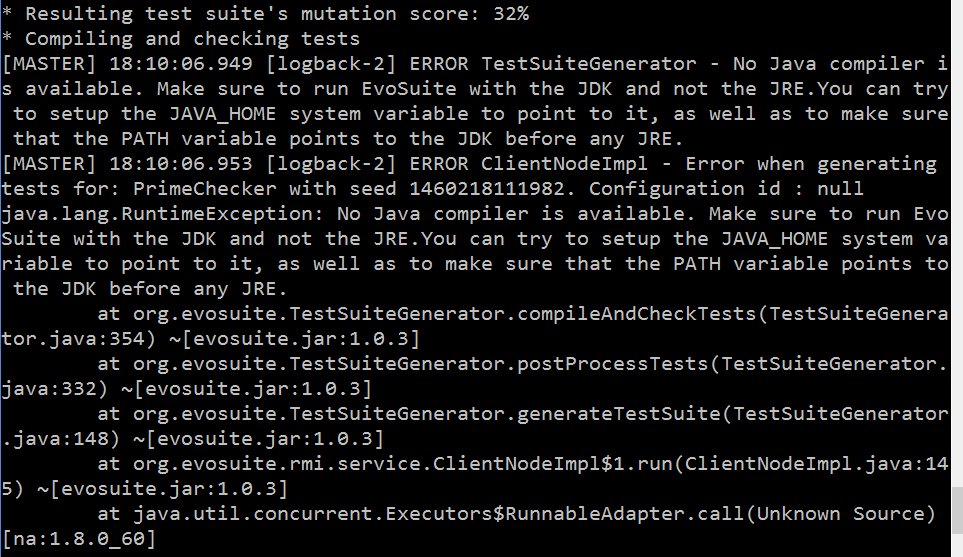
\includegraphics[width=.65\textwidth]{Usability/Error_Evosuite.png}
    \caption{EvoSuite cannot find the Java compiler.}
    \label{fig:error}
    \vspace{.5cm}
\end{figure}

To conclude, a certain set of the environment variables and JDK options did not provide the opportunity for properly set characteristics of the operating system in order to provide the needed scenario to run EvoSuite. 
The absence of detailed documentation and lack of experience resulted in the impossibility of automated test to be generated on the Windows 10 system. 
Nevertheless, when EvoSuite works, it is an effective tool for generating tests to simplify the testing process for developers.
Is a stated solution that will definitely expand its role in the process of automated test generation which will be adopted by software engineers.

\subsection{Maven and EvoSuite}

Generating tests is not all - we need to get these tests to run.
Joda-Time and our own projects made use of Maven as a software project management and comprehension tool. 
Getting EvoSuite dependencies right in the Maven setup is relatively trivial, but it did not work well with other plugins used by the projects.

For example, we integrated Cobertura in each project to calculate branch coverage and cyclomatic complexity. 
Cobertura uses bytecode instrumentation to perform code coverage checks within a class and creates a new class file for the CUT. 
EvoSuite generates tests that are run inside an EvoSuite-dependent sandbox, meaning EvoSuite has its own type of runner. 
When running \verb|mvn corbertura:cobertura| to generate Coberura reports, the tests need to be executed within this sandbox.
The runner attempts to find the CUT but instead runs into two classes: the original CUT, and the class instrumented by Cobertura. 
This confusion causes the JVM to throw a \verb|ClassNotFoundException| and the tests do not get executed. 

To circumvent this problem, it was necessary to manually remove the EvoSuite sandboxing and any EvoSuite dependency within the generated tests. 
Some generated tests used specific EvoSuite assertions to see if an exception was thrown. 
These assertions, unfortunately, had to be removed to generate Cobertura reports. 

\section{Code Snippets}

In this section, we provide code snippets from classes we ran EvoSuite on.

\subsection{PrimeChecker}

\begin{lstlisting}[language=Java, caption=PrimeChecker]
public class PrimeChecker {

    public boolean isPrime(int p) {
        if (p > 1000000000) {
            int max = (int) Math.ceil(Math.sqrt((double) p));

            for (int i = 2; i < max; i++) {
                if ((p % i) == 0) {
                    return false;
                }
            }

            return true;
        } else {
            return false;
        }
    }
}
\end{lstlisting}

\subsection{IntStack}

\begin{lstlisting}[language=Java, caption=IntStack]
public class IntStack {
    private int[] stack;
    private int top_index;

    public IntStack(int capacity) {
        stack = new int[capacity];
        top_index = -1;
    }

    public void push(int i) throws Exception {
        if (!isFull()) {
            int new_top_index = top_index + 1;
            stack[new_top_index] = i;
            top_index = new_top_index;
        } else {
            throw new Exception("Stack is full");
        }
    }

    public int pop() throws Exception {
        if(!isEmpty()) {
            int i = peek();
            top_index = top_index - 1;
            return i;
        } else {
            throw new Exception("Stack is empty");
        }
    }

    public int peek() throws Exception {
        if (!isEmpty()) {
            return stack[top_index];
        } else {
            throw new Exception("Stack is empty");
        }
    }

    public boolean isEmpty() {
        return top_index == -1;
    }

    public boolean isFull() {
        return top_index == capacity() - 1;
    }

    public int capacity() {
        return stack.length;
    }
}
\end{lstlisting}

\subsection{ColourPicker}

\begin{lstlisting}[language=Java, caption=ColourPicker]
public class ColourPicker {

    public Color toColor(boolean number, int i, String name) {
        if (number) {
            if (i == 0) {
                return Color.WHITE;
            } else if (i == 1) {
                return Color.RED;
            } else if (i == 2) {
                return Color.GREEN;
            } else if (i == 3) {
                return Color.BLUE;
            } else if (i == 4) {
                return Color.MAGENTA;
            } else if (i == 5) {
                return Color.YELLOW;
            } else if (i == 6) {
                return Color.CYAN;
            } else {
                return Color.BLACK;
            }
        } else {
            switch (name) {
                case "red" : return Color.RED;
                case "green" : return Color.GREEN;
                case "blue" : return Color.BLUE;
                case "yellow" : return Color.MAGENTA;
                case "magenta" : return Color.YELLOW;
                case "cyan" : return Color.CYAN;
                default : if(i == 0) {
                    return Color.WHITE;
                } else {
                    return Color.BLACK;
                }
            }
        }
    }

    public Color pickRGB() {
        Random rnd = new Random();
        int i = rnd.nextInt() * 10;

        if (i < 4) {
            return Color.RED;
        } else if (i < 7) {
            return Color.GREEN;
        } else {
            return Color.BLUE;
        }
    }
}
\end{lstlisting}

\subsection{EnglishNumberToWords}

Source: \url{http://www.rgagnon.com/javadetails/java-0426.html}.
\begin{lstlisting}[language=Java, caption=EnglishNumberToWords]
public class EnglishNumberToWords {
	private static final String[] tensNames = {
			"",
			" ten",
			" twenty",
			" thirty",
			" forty",
			" fifty",
			" sixty",
			" seventy",
			" eighty",
			" ninety"
	};

	private static final String[] numNames = {
			"",
			" one",
			" two",
			" three",
			" four",
			" five",
			" six",
			" seven",
			" eight",
			" nine",
			" ten",
			" eleven",
			" twelve",
			" thirteen",
			" fourteen",
			" fifteen",
			" sixteen",
			" seventeen",
			" eighteen",
			" nineteen"
	};

	private EnglishNumberToWords() {}

	private static String convertLessThanOneThousand(int number) {
		String soFar;

		if (number % 100 < 20){
			soFar = numNames[number % 100];
			number /= 100;
		}
		else {
			soFar = numNames[number % 10];
			number /= 10;

			soFar = tensNames[number % 10] + soFar;
			number /= 10;
		}
		if (number == 0) return soFar;
		return numNames[number] + " hundred" + soFar;
	}


	public static String convert(long number) {
		// 0 to 999 999 999 999
		if (number == 0) { return "zero"; }

		String snumber = Long.toString(number);

		// pad with "0"
		String mask = "000000000000";
		DecimalFormat df = new DecimalFormat(mask);
		snumber = df.format(number);

		// XXXnnnnnnnnn
		int billions = Integer.parseInt(snumber.substring(0,3));
		// nnnXXXnnnnnn
		int millions  = Integer.parseInt(snumber.substring(3,6));
		// nnnnnnXXXnnn
		int hundredThousands = Integer.parseInt(snumber.substring(6,9));
		// nnnnnnnnnXXX
		int thousands = Integer.parseInt(snumber.substring(9,12));

		String tradBillions;
		switch (billions) {
			case 0:
				tradBillions = "";
				break;
			case 1 :
				tradBillions = convertLessThanOneThousand(billions)
						+ " billion ";
				break;
			default :
				tradBillions = convertLessThanOneThousand(billions)
						+ " billion ";
		}
		String result =  tradBillions;

		String tradMillions;
		switch (millions) {
			case 0:
				tradMillions = "";
				break;
			case 1 :
				tradMillions = convertLessThanOneThousand(millions)
						+ " million ";
				break;
			default :
				tradMillions = convertLessThanOneThousand(millions)
						+ " million ";
		}
		result =  result + tradMillions;

		String tradHundredThousands;
		switch (hundredThousands) {
			case 0:
				tradHundredThousands = "";
				break;
			case 1 :
				tradHundredThousands = "one thousand ";
				break;
			default :
				tradHundredThousands = convertLessThanOneThousand(hundredThousands)
						+ " thousand ";
		}
		result =  result + tradHundredThousands;

		String tradThousand;
		tradThousand = convertLessThanOneThousand(thousands);
		result =  result + tradThousand;

		// remove extra spaces!
		return result.replaceAll("^\\s+", "").replaceAll("\\b\\s{2,}\\b", " ");
	}
}
\end{lstlisting}
